% THIS IS SIGPROC-SP.TEX - VERSION 3.1
% WORKS WITH V3.2SP OF ACM_PROC_ARTICLE-SP.CLS
% APRIL 2009
%
% It is an example file showing how to use the 'acm_proc_article-sp.cls' V3.2SP
% LaTeX2e document class file for Conference Proceedings submissions.
% ----------------------------------------------------------------------------------------------------------------
% This .tex file (and associated .cls V3.2SP) *DOES NOT* produce:
%       1) The Permission Statement
%       2) The Conference (location) Info information
%       3) The Copyright Line with ACM data
%       4) Page numbering
% ---------------------------------------------------------------------------------------------------------------
% It is an example which *does* use the .bib file (from which the .bbl file
% is produced).
% REMEMBER HOWEVER: After having produced the .bbl file,
% and prior to final submission,
% you need to 'insert'  your .bbl file into your source .tex file so as to provide
% ONE 'self-contained' source file.
%
% Questions regarding SIGS should be sent to
% Adrienne Griscti ---> griscti@acm.org
%
% Questions/suggestions regarding the guidelines, .tex and .cls files, etc. to
% Gerald Murray ---> murray@hq.acm.org
%
% For tracking purposes - this is V3.1SP - APRIL 2009

\documentclass{acm_proc_article-sp}
\usepackage{ctex}[utf8]
\usepackage{float}
\usepackage{listings}
\begin{document}

\title{Project 2 实验报告}
%
% You need the command \numberofauthors to handle the 'placement
% and alignment' of the authors beneath the title.
%
% For aesthetic reasons, we recommend 'three authors at a time'
% i.e. three 'name/affiliation blocks' be placed beneath the title.
%
% NOTE: You are NOT restricted in how many 'rows' of
% "name/affiliations" may appear. We just ask that you restrict
% the number of 'columns' to three.
%
% Because of the available 'opening page real-estate'
% we ask you to refrain from putting more than six authors
% (two rows with three columns) beneath the article title.
% More than six makes the first-page appear very cluttered indeed.
%
% Use the \alignauthor commands to handle the names
% and affiliations for an 'aesthetic maximum' of six authors.
% Add names, affiliations, addresses for
% the seventh etc. author(s) as the argument for the
% \additionalauthors command.
% These 'additional authors' will be output/set for you
% without further effort on your part as the last section in
% the body of your article BEFORE References or any Appendices.

\numberofauthors{2} %  in this sample file, there are a *total*
% of EIGHT authors. SIX appear on the 'first-page' (for formatting
% reasons) and the remaining two appear in the \additionalauthors section.
%
\author{
% You can go ahead and credit any number of authors here,
% e.g. one 'row of three' or two rows (consisting of one row of three
% and a second row of one, two or three).
%
% The command \alignauthor (no curly braces needed) should
% precede each author name, affiliation/snail-mail address and
% e-mail address. Additionally, tag each line of
% affiliation/address with \affaddr, and tag the
% e-mail address with \email.
%
% 1st. author
\alignauthor
曾正 \\
软71 \\
2017011438
}
% There's nothing stopping you putting the seventh, eighth, etc.
% author on the opening page (as the 'third row') but we ask,
% for aesthetic reasons that you place these 'additional authors'
% in the \additional authors block, viz.

% Just remember to make sure that the TOTAL number of authors
% is the number that will appear on the first page PLUS the
% number that will appear in the \additionalauthors section.

\maketitle
\begin{abstract}
实验报告介绍了银行精准营销解决方案和青蛙叫声聚类分析的实现说明以及实验结果等。
\end{abstract}

\keywords{Classification, NBC, Clustering, K-Means} % NOT required for Proceedings

\section{银行精准营销解决方案}
\subsection{使用说明}
环境依赖
\begin{lstlisting}
pip install sklearn pandas numpy
\end{lstlisting}

运行方式
\begin{lstlisting}
python classification.py
\end{lstlisting}
启动后会自动开始训练模型进行分类并输出分类结果。

\subsection{分类器模型}
\begin{itemize}
    \item NaiveBayesClassifier(朴素贝叶斯分类器):自行实现。\\
    分类器原理:有贝叶斯定理如下:
    $$P(A|B) = \frac{P(A|B)P(B)}{P(A)}$$
    由此我们可得到:
    $$P(Cla|Fea)=\frac{P(Fea|Cla)P(Cla)}{P(Fea)}$$
    利用上述公式我们就很容易求得目标$$P(Cla|Fea)$$,即在给定特征集合(Features)的条件下,属于某一类别(Class)的概率。需要注意的是在贝叶斯定理中,有假设:特征集合(Features)中各特征相互独立。有如上假设便可得:\\ \\
    $P(Cla|Feas)=\frac{P(FeaA|Cla)P(Cla)*P(FeaB|Cla)P(Cla)}{P(Feas)}$ \\ \\
    再根据中心极限定理,在样本数量足够大时,频率等于概率。

    以上便构成了实现朴素贝叶斯分类器的基本原理,基于上述原理很容易就可以实现朴素贝叶斯分类器。

    \item RandomForestClassifier(随机森林分类器):调用sklearn库,使用默认参数。
    \item GradientBoostingClassifier(梯度提升树分类器):调用sklearn库,使用默认参数。
\end{itemize}

\subsection{特征组合选择}
首先由于特征ID与客户信息完全无关,且数据集y=1集中在后面,会对分类结果造成较大负面影响,故将特其去除,其次注意到特征Default中大部分数据缺失,不具有参考价值,故也去除。之后分为以下两组特征组合:
\begin{itemize}
    \item 从客户的个人信息入手进行分析。考虑客户的年龄、工作、受教育程度、婚姻等会影响客户财产状况及理财思维的因素,构成特征组合:["age", "job", "marital", "education", "balance", "housing", "loan"]
    \item 从银行客服与用户的联系频率及效果入手进行分析。首先去除Month、Day,这是由于缺乏年份,无法确定时间的早晚。剩余特征便可构成银行与客户沟通相关的特征组合:["contact", "duration", "campaign", "pdays", "previous", "poutcome"]
\end{itemize}

\subsection{模型验证}
由于提供的数据集全部为有标数据,因此采用了K-折交叉验证的方法。考虑到数据集大小,此处采用的是10折交叉验证,即将全部数据集十等分,依次将每一份作为测试集,剩余$9/10$用作训练集通过比较结果从而验证模型的可靠性。考虑到前面提到的数据集特征y的有序性,故在读入数据时首先进行了乱序。
\subsection{评价指标}
评价指标采用分类正确率的大小进行比较,其范围为$[0, 1]$。
\subsection{分类效果差异及其原因}
某一次训练的分类结果如下:\\
\begin{tabular}{cccc}
分类器(组合1)&RFC&GBC&NBC \\
1&0.872&0.879&0.669 \\
2&0.871&0.883&0.662 \\
3&0.877&0.889&0.665 \\
4&0.863&0.870&0.655 \\
5&0.872&0.887&0.651 \\
6&0.863&0.872&0.665 \\
7&0.870&0.884&0.635 \\
8&0.866&0.882&0.659 \\
9&0.875&0.887&0.655 \\
10&0.867&0.881&0.667
\end{tabular}

\begin{tabular}{cccc}
分类器(组合2)&RFC&GBC&NBC \\
1&0.882&0.904&0.795 \\
2&0.890&0.913&0.789 \\
3&0.890&0.913&0.796 \\
4&0.878&0.893&0.789 \\
5&0.898&0.909&0.790 \\
6&0.877&0.890&0.793 \\
7&0.879&0.902&0.781 \\
8&0.887&0.911&0.796 \\
9&0.894&0.907&0.789 \\
10&0.882&0.900&0.781
\end{tabular}

从上述数据我们可以得到两个较为明显的特征:
\begin{itemize}
    \item 分类器分类效果:GBC > RFC > NBC
    \item 特征组合分类效果:组合2 > 组合1,其中RFC和GBC收到影响较小,对NBC影响很大。
\end{itemize}
原因分析:

GBC和RFC的分类效果接近,均达到0.88左右,相比之下NBC的表现就要差了不少,组合2有0.79左右正确率,而组合1时仅有0.65左右的正确率。关于这一点根据前面提到的朴素贝叶斯分类器的基本原理我们很容易找到原因,贝叶斯定理的前提条件是,特征组合的各个特征之间需要相互独立。而在我们所选择的无论组合一还是组合二都很容易发现它们彼此之间并非是完全独立的,例如组合二中的Campaign(在本次活动中,与该客户交流过的次数)就和Duration(最后一次联系的交流时长)可能存在一些关系,即两者之间并不独立。基于这一点就很容易理解为何NBC的分类效果较差。

对于特征二我们可以从之前选择特征组合的出发点进行考虑。组合一是客户的个人特征,几乎与银行无关,而组合二则是客户与银行、与该产品都相关的重要信息。此外,加上各特征间的独立性增强,因此在由组合一到组合二时,NBC的正确率得到了很大的提升。相比之下,GBC和RFC由于正确率已经达到了其自身分类能力的阈值故正确率较难得到很大的增长。

\section{青蛙叫声聚类分析}
\subsection{使用说明}
环境依赖
\begin{lstlisting}
pip install matplotlib
\end{lstlisting}

运行方式
\begin{lstlisting}
python clustering.py
\end{lstlisting}
启动后会自动开始训练模型进行聚类并展示可视化聚类结果。

\subsection{分类器模型}
\begin{itemize}
    \item K-Means:自行实现。\\
    K-Means聚类算法的基本思想很简单,就是将全部数据划分为k个簇(Cluster),使得簇内的各点间尽可能紧密连接在一起,而簇间的距离尽可能地大。\\
    基于上述基本思想我们首先将全部数据划分为$C_1, C_2,..., C_k$,给个簇的质心分别为$\mu_1, \mu_2,..., \mu_k$,其表达式为
    $$\mu_i = \frac{\sum\limits_{x \in C_i}x}{|C_i|}$$
    利用上式,我们可以得到平方误差为
    $$E=\sum\limits_{i=1}^{k}\sum\limits_{x \in C_i}||x - \mu_i||_2^2$$
    这样我们的目标就变成了求解E的最小值,但是这是一个NP-hard,故采用启发式的迭代过程。\\
    首先随机选取k个簇的质心,计算所有点到该质心距离,比较距离取较小者即可得到首次迭代后的簇划分。之后便可求得各簇的质心,之后重复上述过程直到簇不再改变。\\
    按照上述原理我们便可以实现K-Means聚类模型。
    \item Birch:调用sklearn库,$n\_cluster=k$。
\end{itemize}

\subsection{特征组合选择}
特征组合的选取采用了两种方式:
\begin{itemize}
    \item 手动选取:MFCC的各个特征量间并没有明显的主次之分,可以考虑随机选取。此处是选择最后5个特征量。
    \item 使用PCA降维,减少特征量。
\end{itemize}

\subsection{距离度量及超参数选择}
\begin{itemize}
    \item 距离度量:采用欧几里得距离。
    \item 超参数选择:K-Means和Birch的超参数均为k,这里k的确定是通过计算$k = [2, 6]$时得到的轮廓系数大小进行比较,选取轮廓系数较大的k作为超参数。但注意到此次聚类是对青蛙所属的科(Family)进行聚类比较,共四科,故$k = 4$
\end{itemize}
\begin{figure}[H]
    \centering
    \caption{$k-SilScore$}
    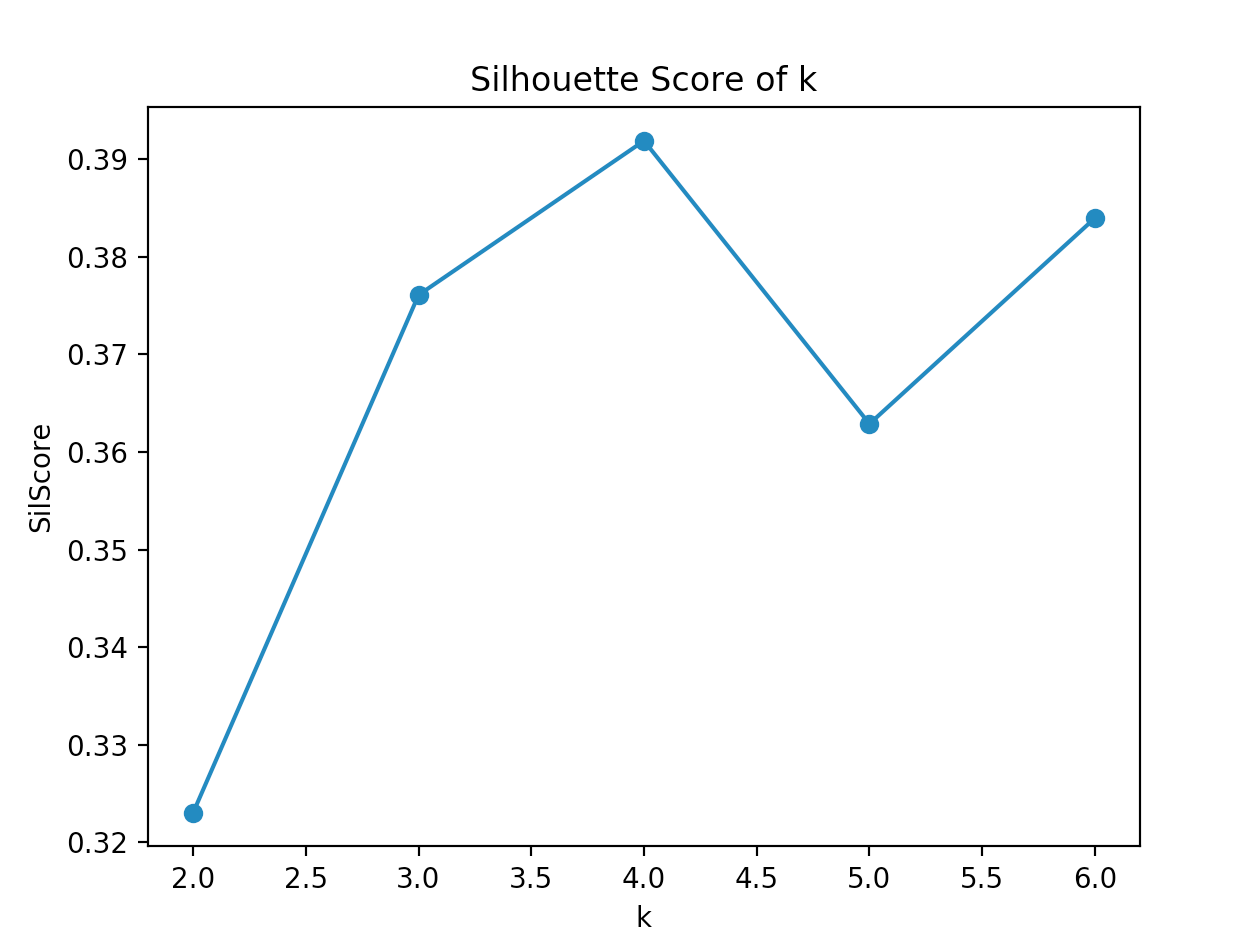
\includegraphics[width=0.4\textwidth]{k.png}
\end{figure}
次数选择$k = 4$

\subsection{评价指标}
\begin{itemize}
    \item Calinski-Harabaz Index(CH指标):\\
    $$CH(k) = \frac{trB(k)/(k - 1)}{trW(k)/(n - k)}$$
    故CH指标越大簇自身越紧密,簇与簇之间越分散,聚类结果越好。
    \item Silhouette Coefficient(轮廓系数):\\
    $$s(i) = \frac{b(i) - a(i)}{max\{a(i), b(i)\}}$$
    故轮廓系数越接近$1$聚类效果越好,越接近$-1$结果越差
\end{itemize}
\subsection{聚类效果差异及其原因}
\begin{itemize}
    \item Birch,特征组合1。CH指标: 6540.1,轮廓系数: 0.389 
    \begin{figure}[H]
        \centering
        \caption{$Birch-1$}
        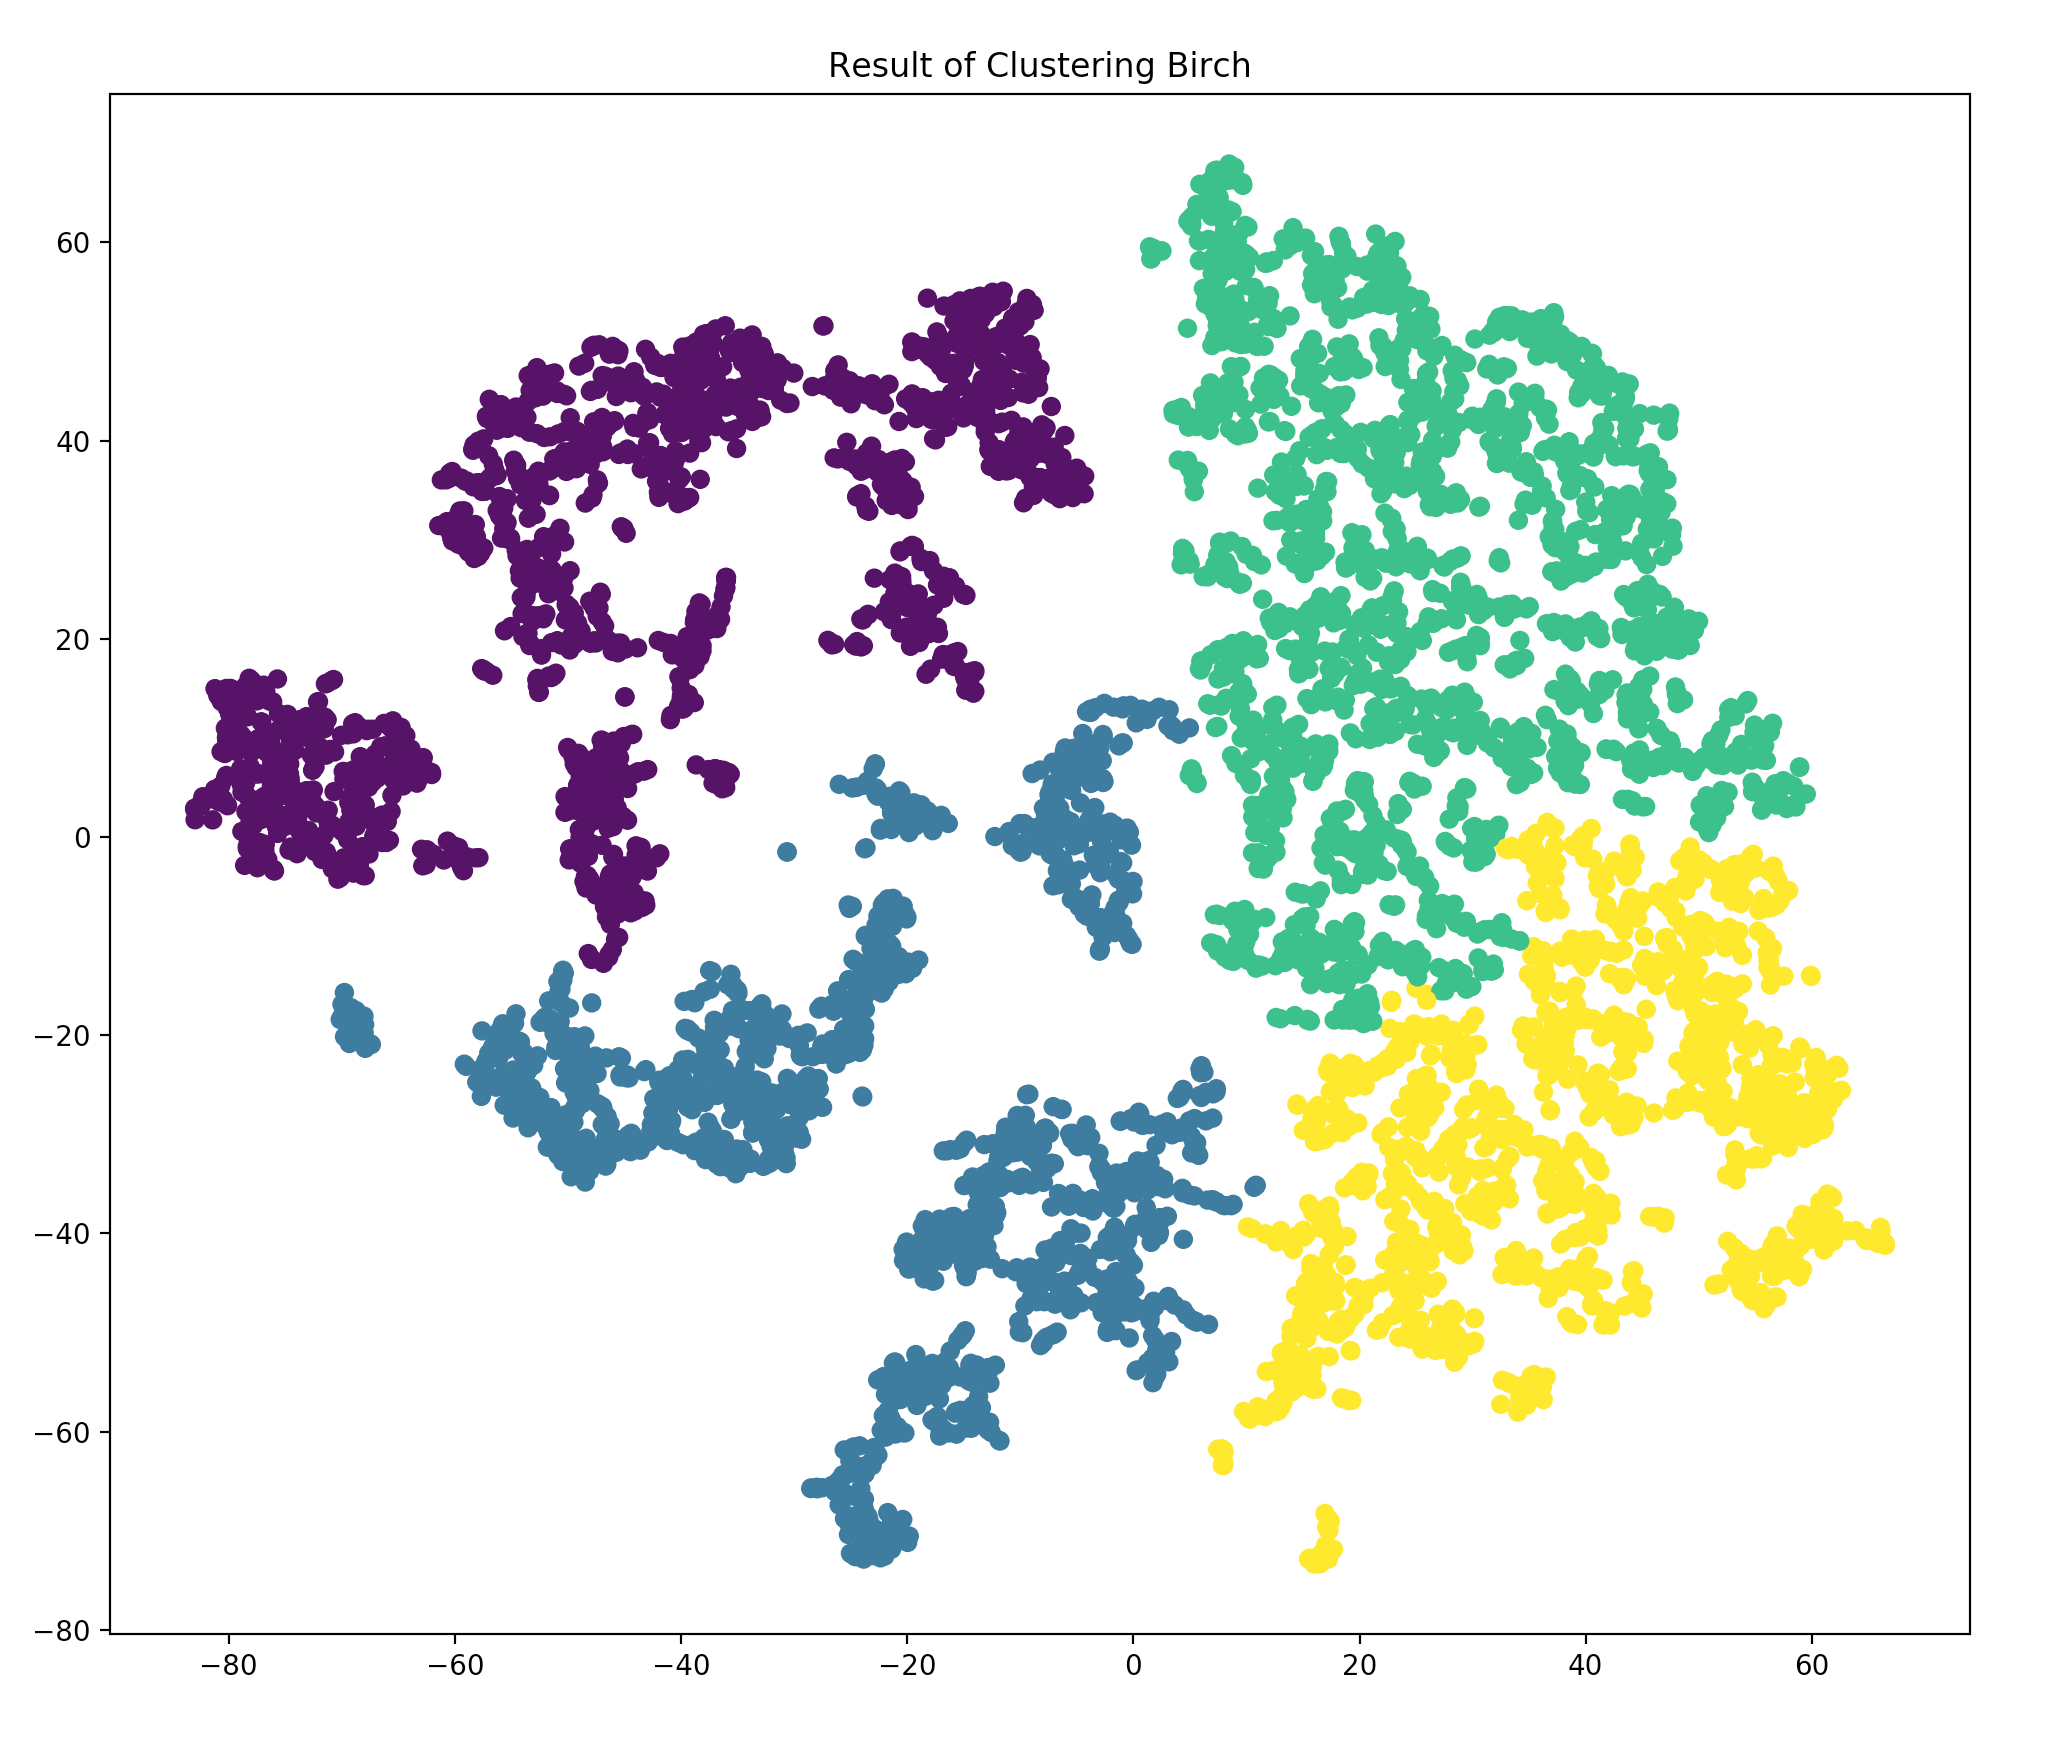
\includegraphics[width=0.4\textwidth]{1-1.png}
    \end{figure}
    \item K-Means,特征组合1。CH指标: 7377.3,轮廓系数: 0.414 
    \begin{figure}[H]
        \centering
        \caption{$KMeans-1$}
        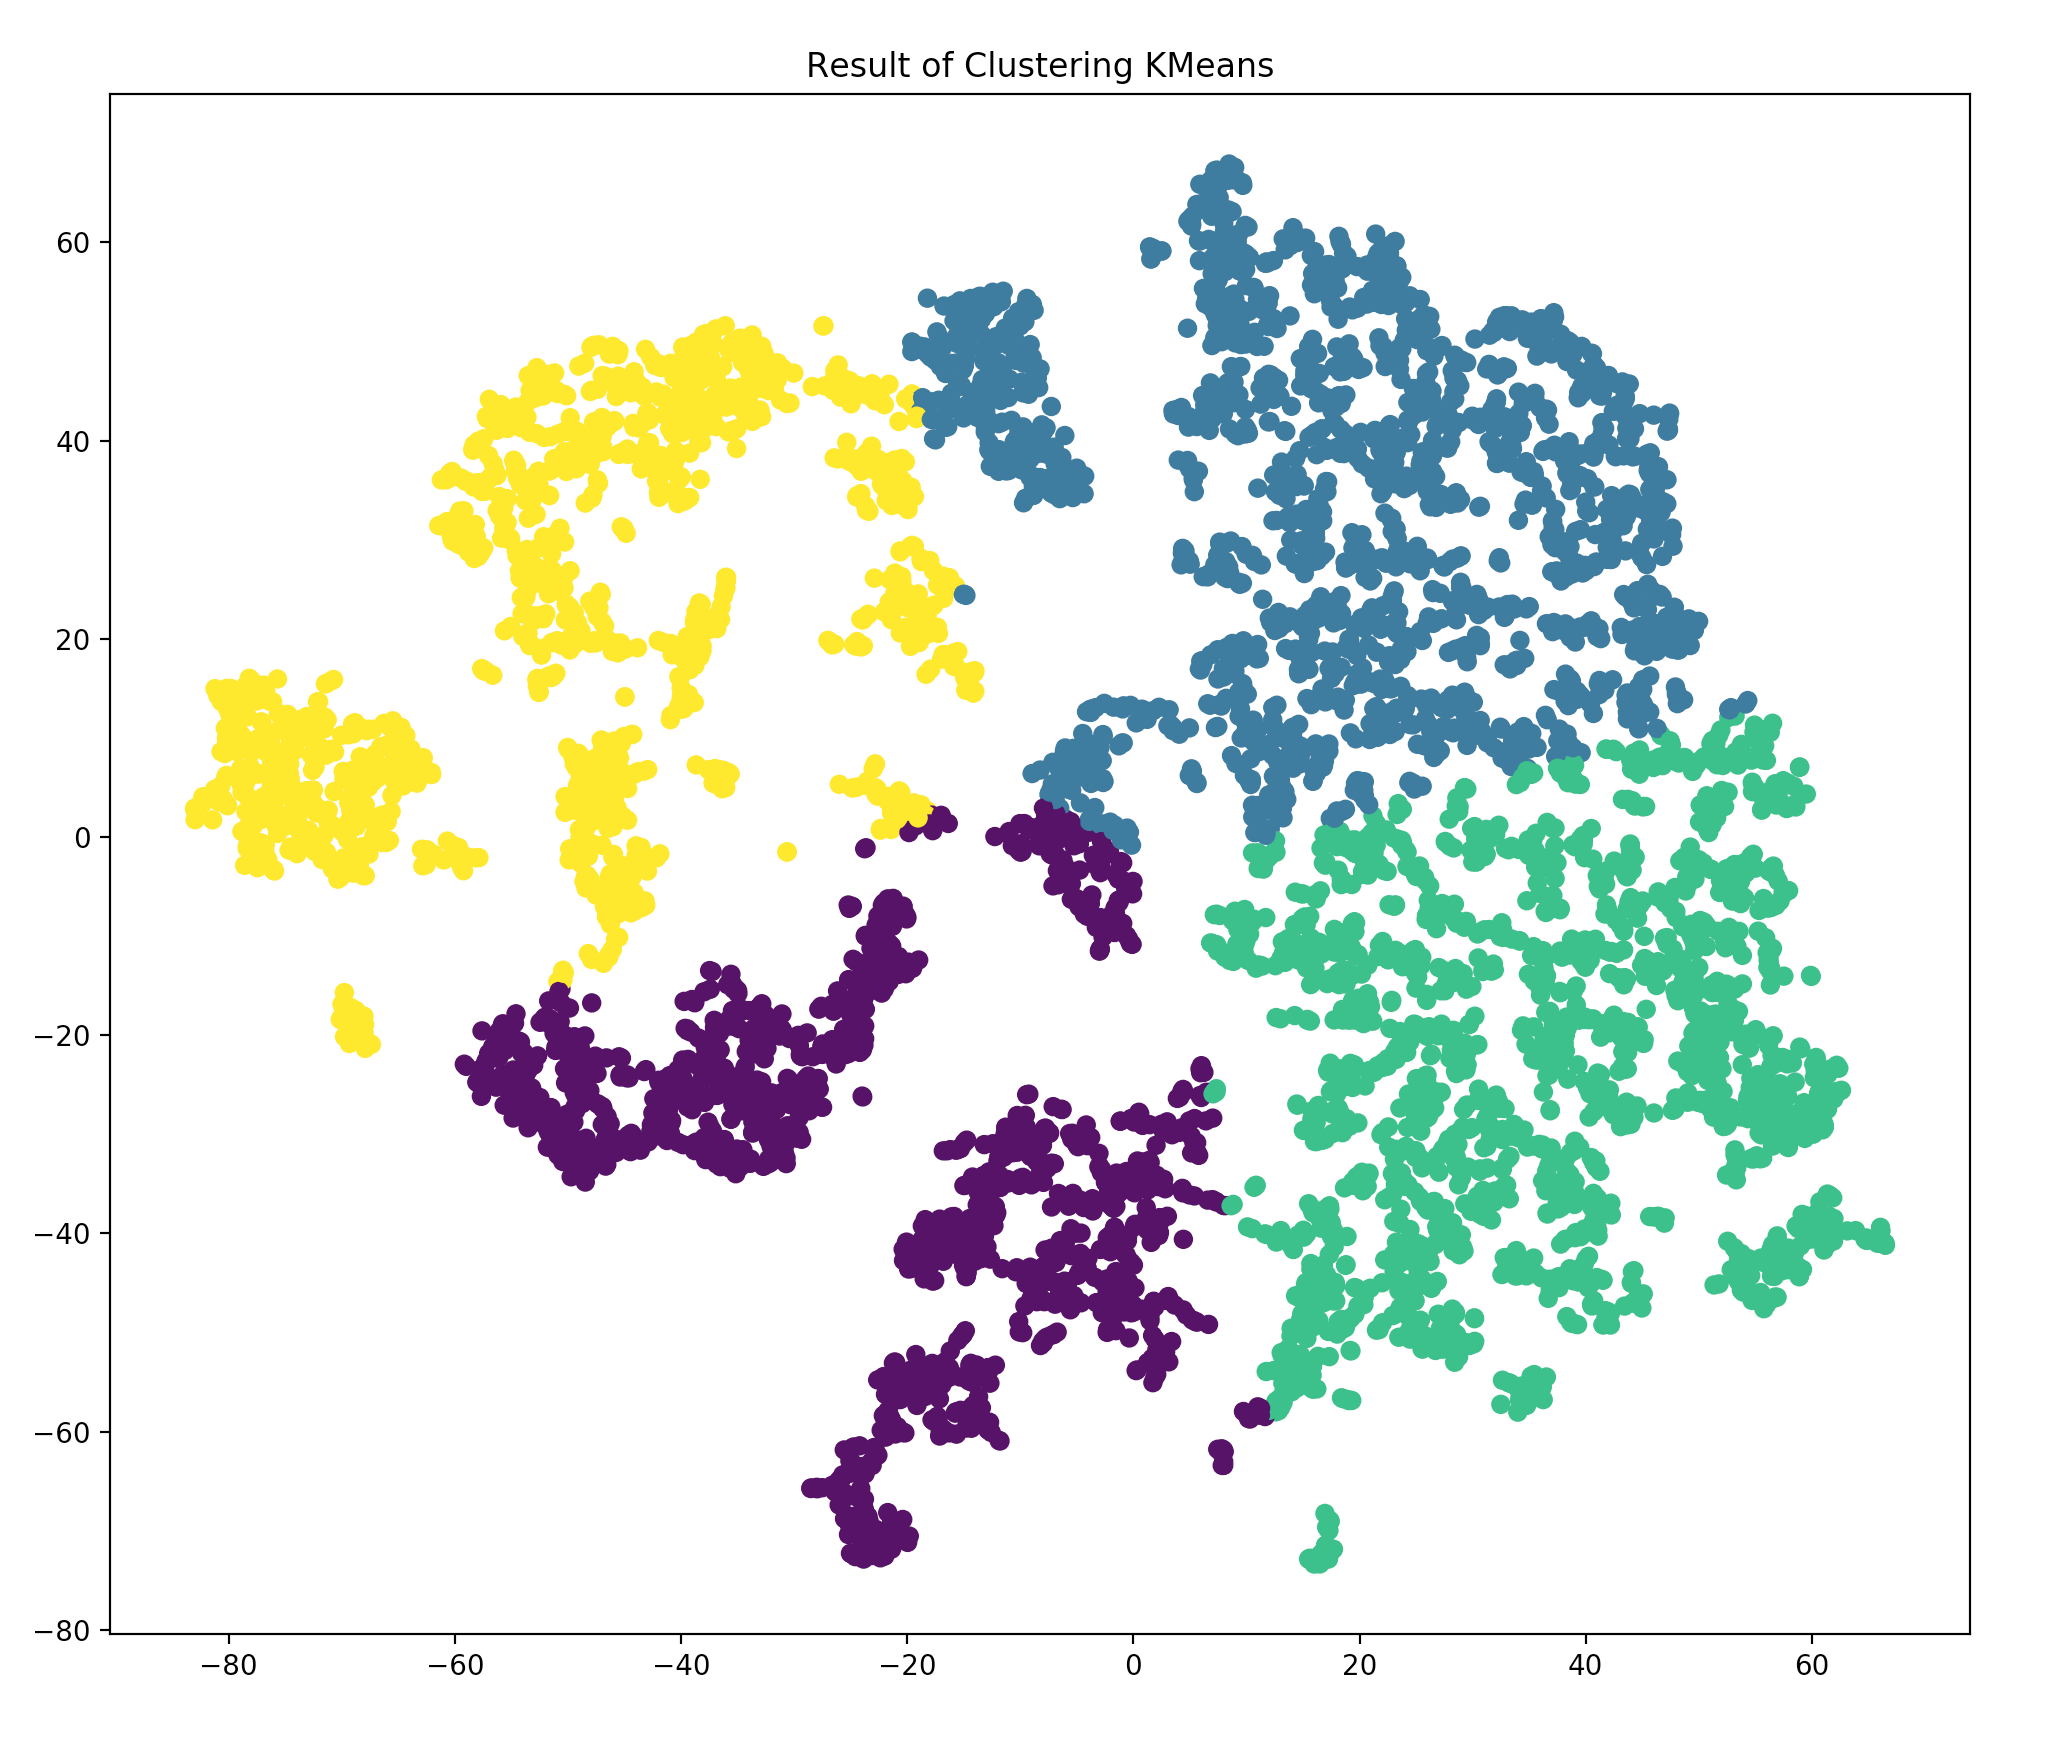
\includegraphics[width=0.4\textwidth]{1-2.png}
    \end{figure}
    \item Birch,特征组合2。CH指标: 722.4,轮廓系数: 0.416 
    \begin{figure}[H]
        \centering
        \caption{$Birch-2$}
        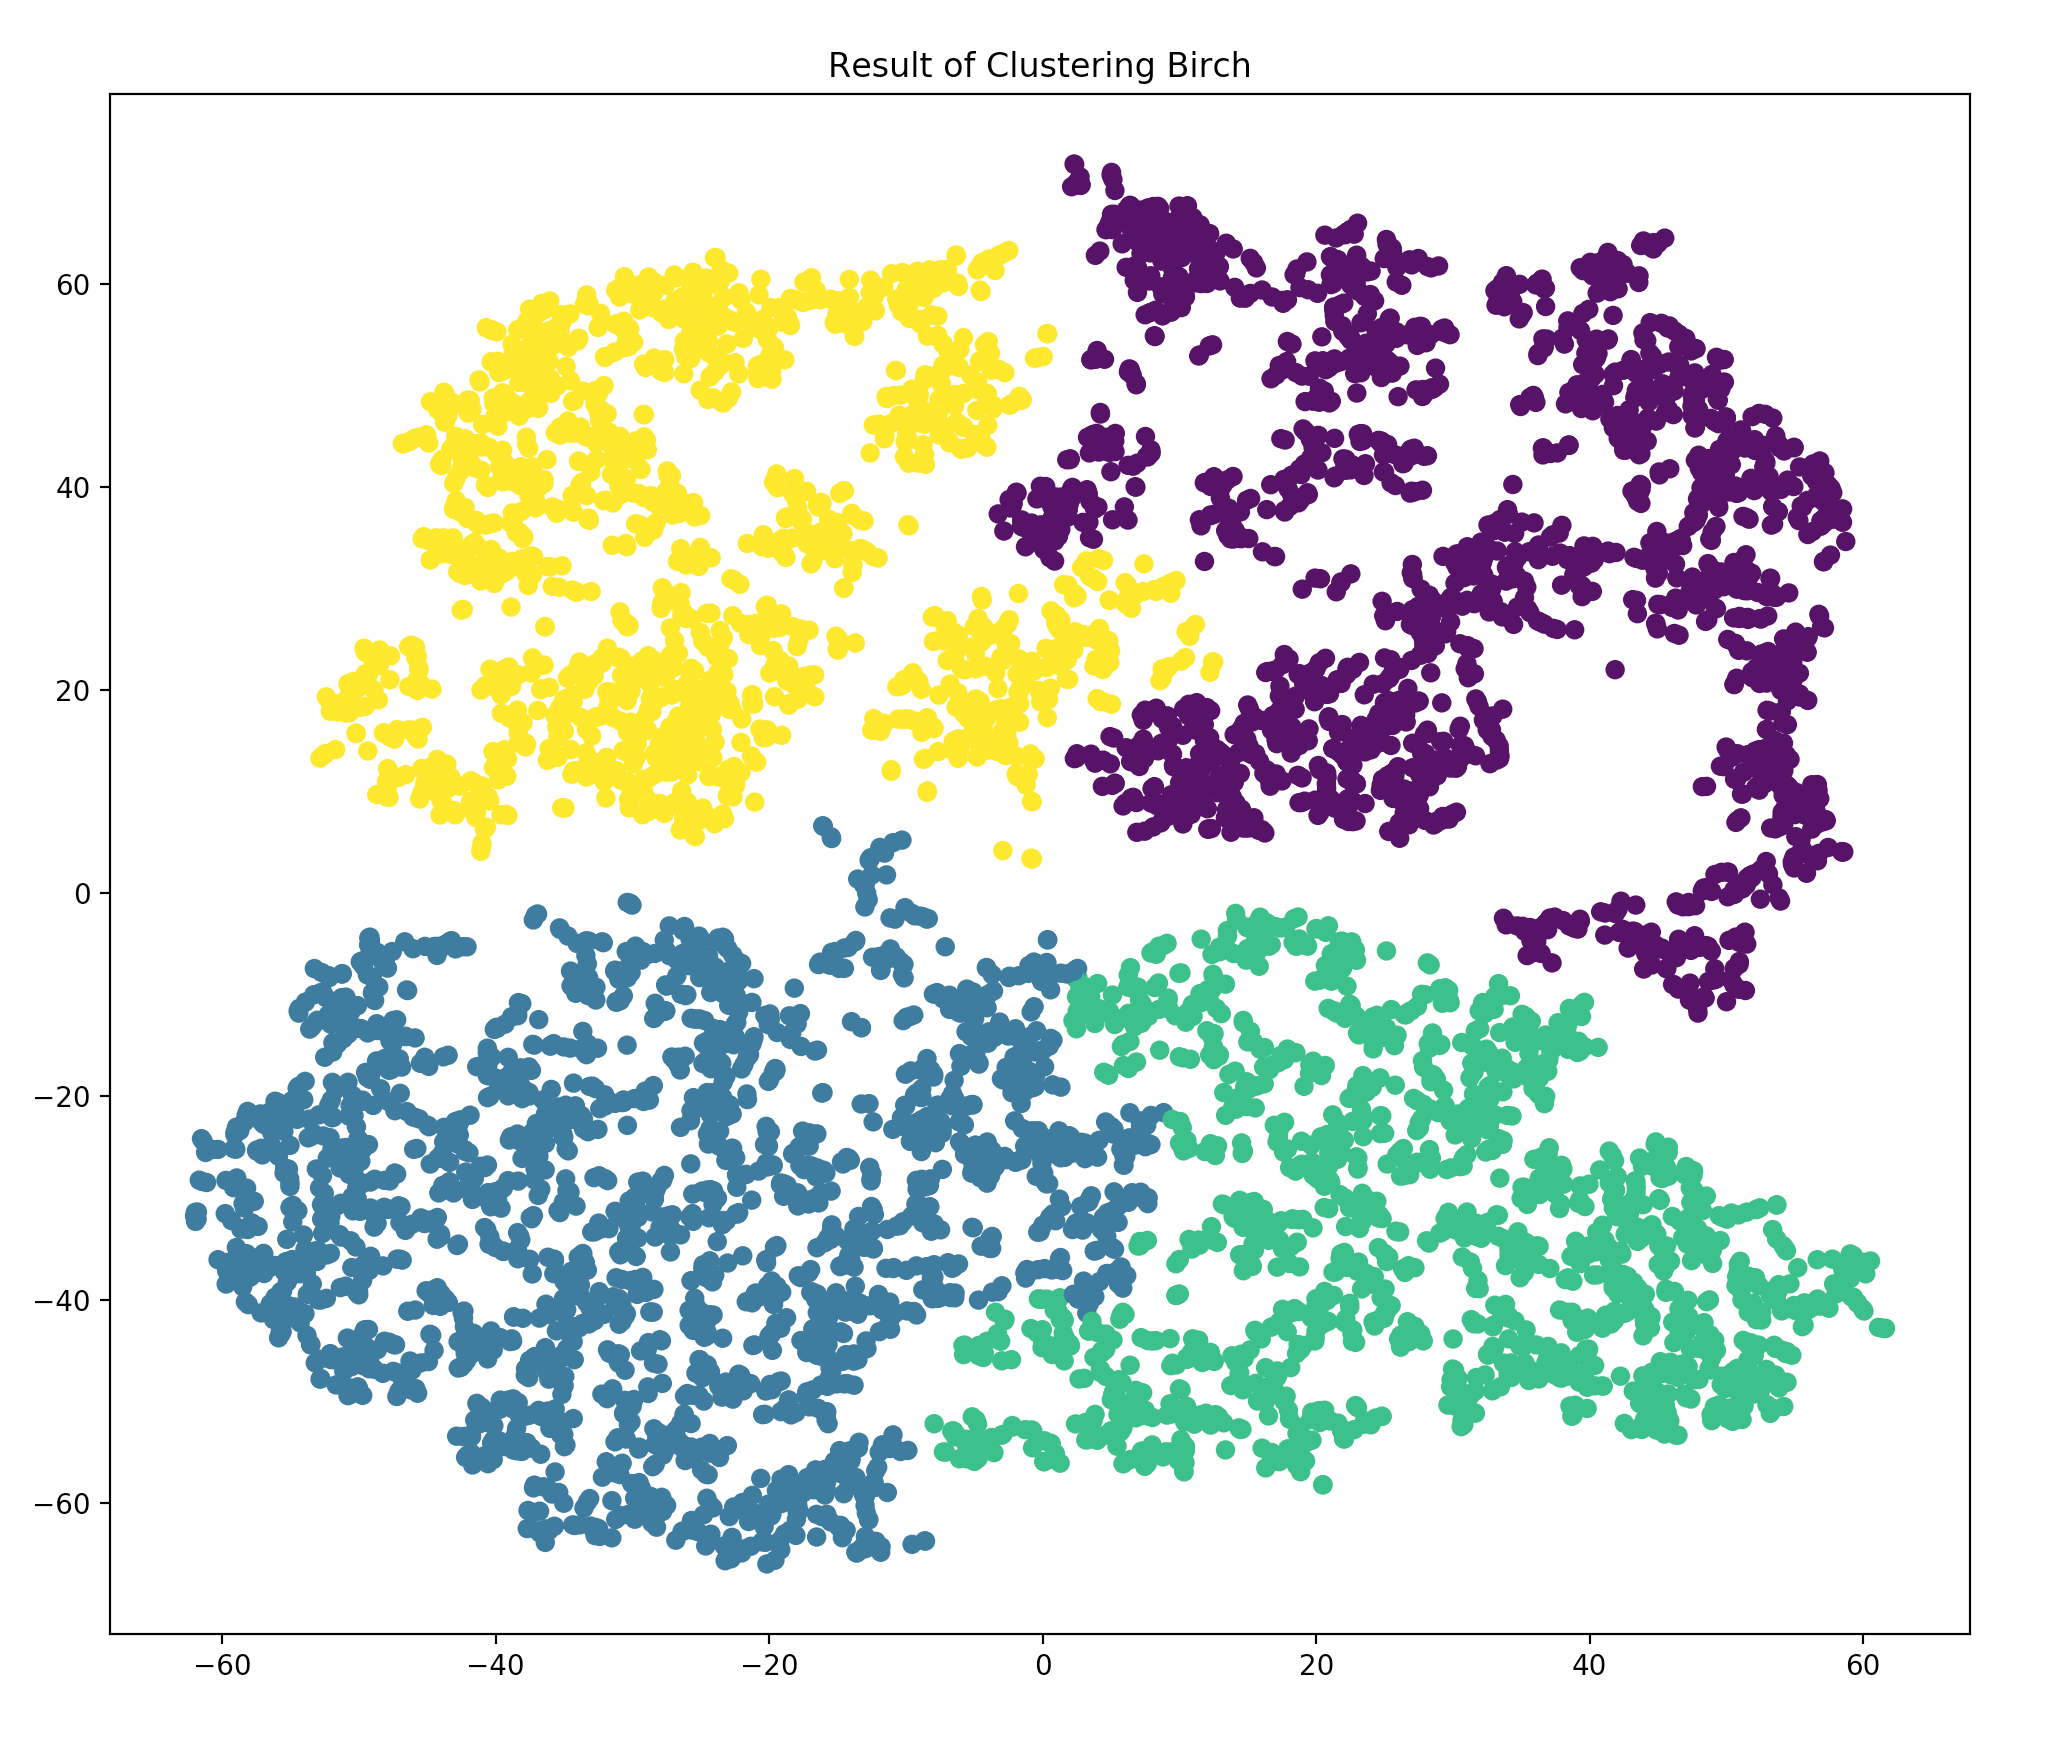
\includegraphics[width=0.4\textwidth]{2-1.png}
    \end{figure}
    \item K-Means,特征组合2。CH指标: 8317.9,轮廓系数: 0.441 
    \begin{figure}[H]
        \centering
        \caption{$KMeans-2$}
        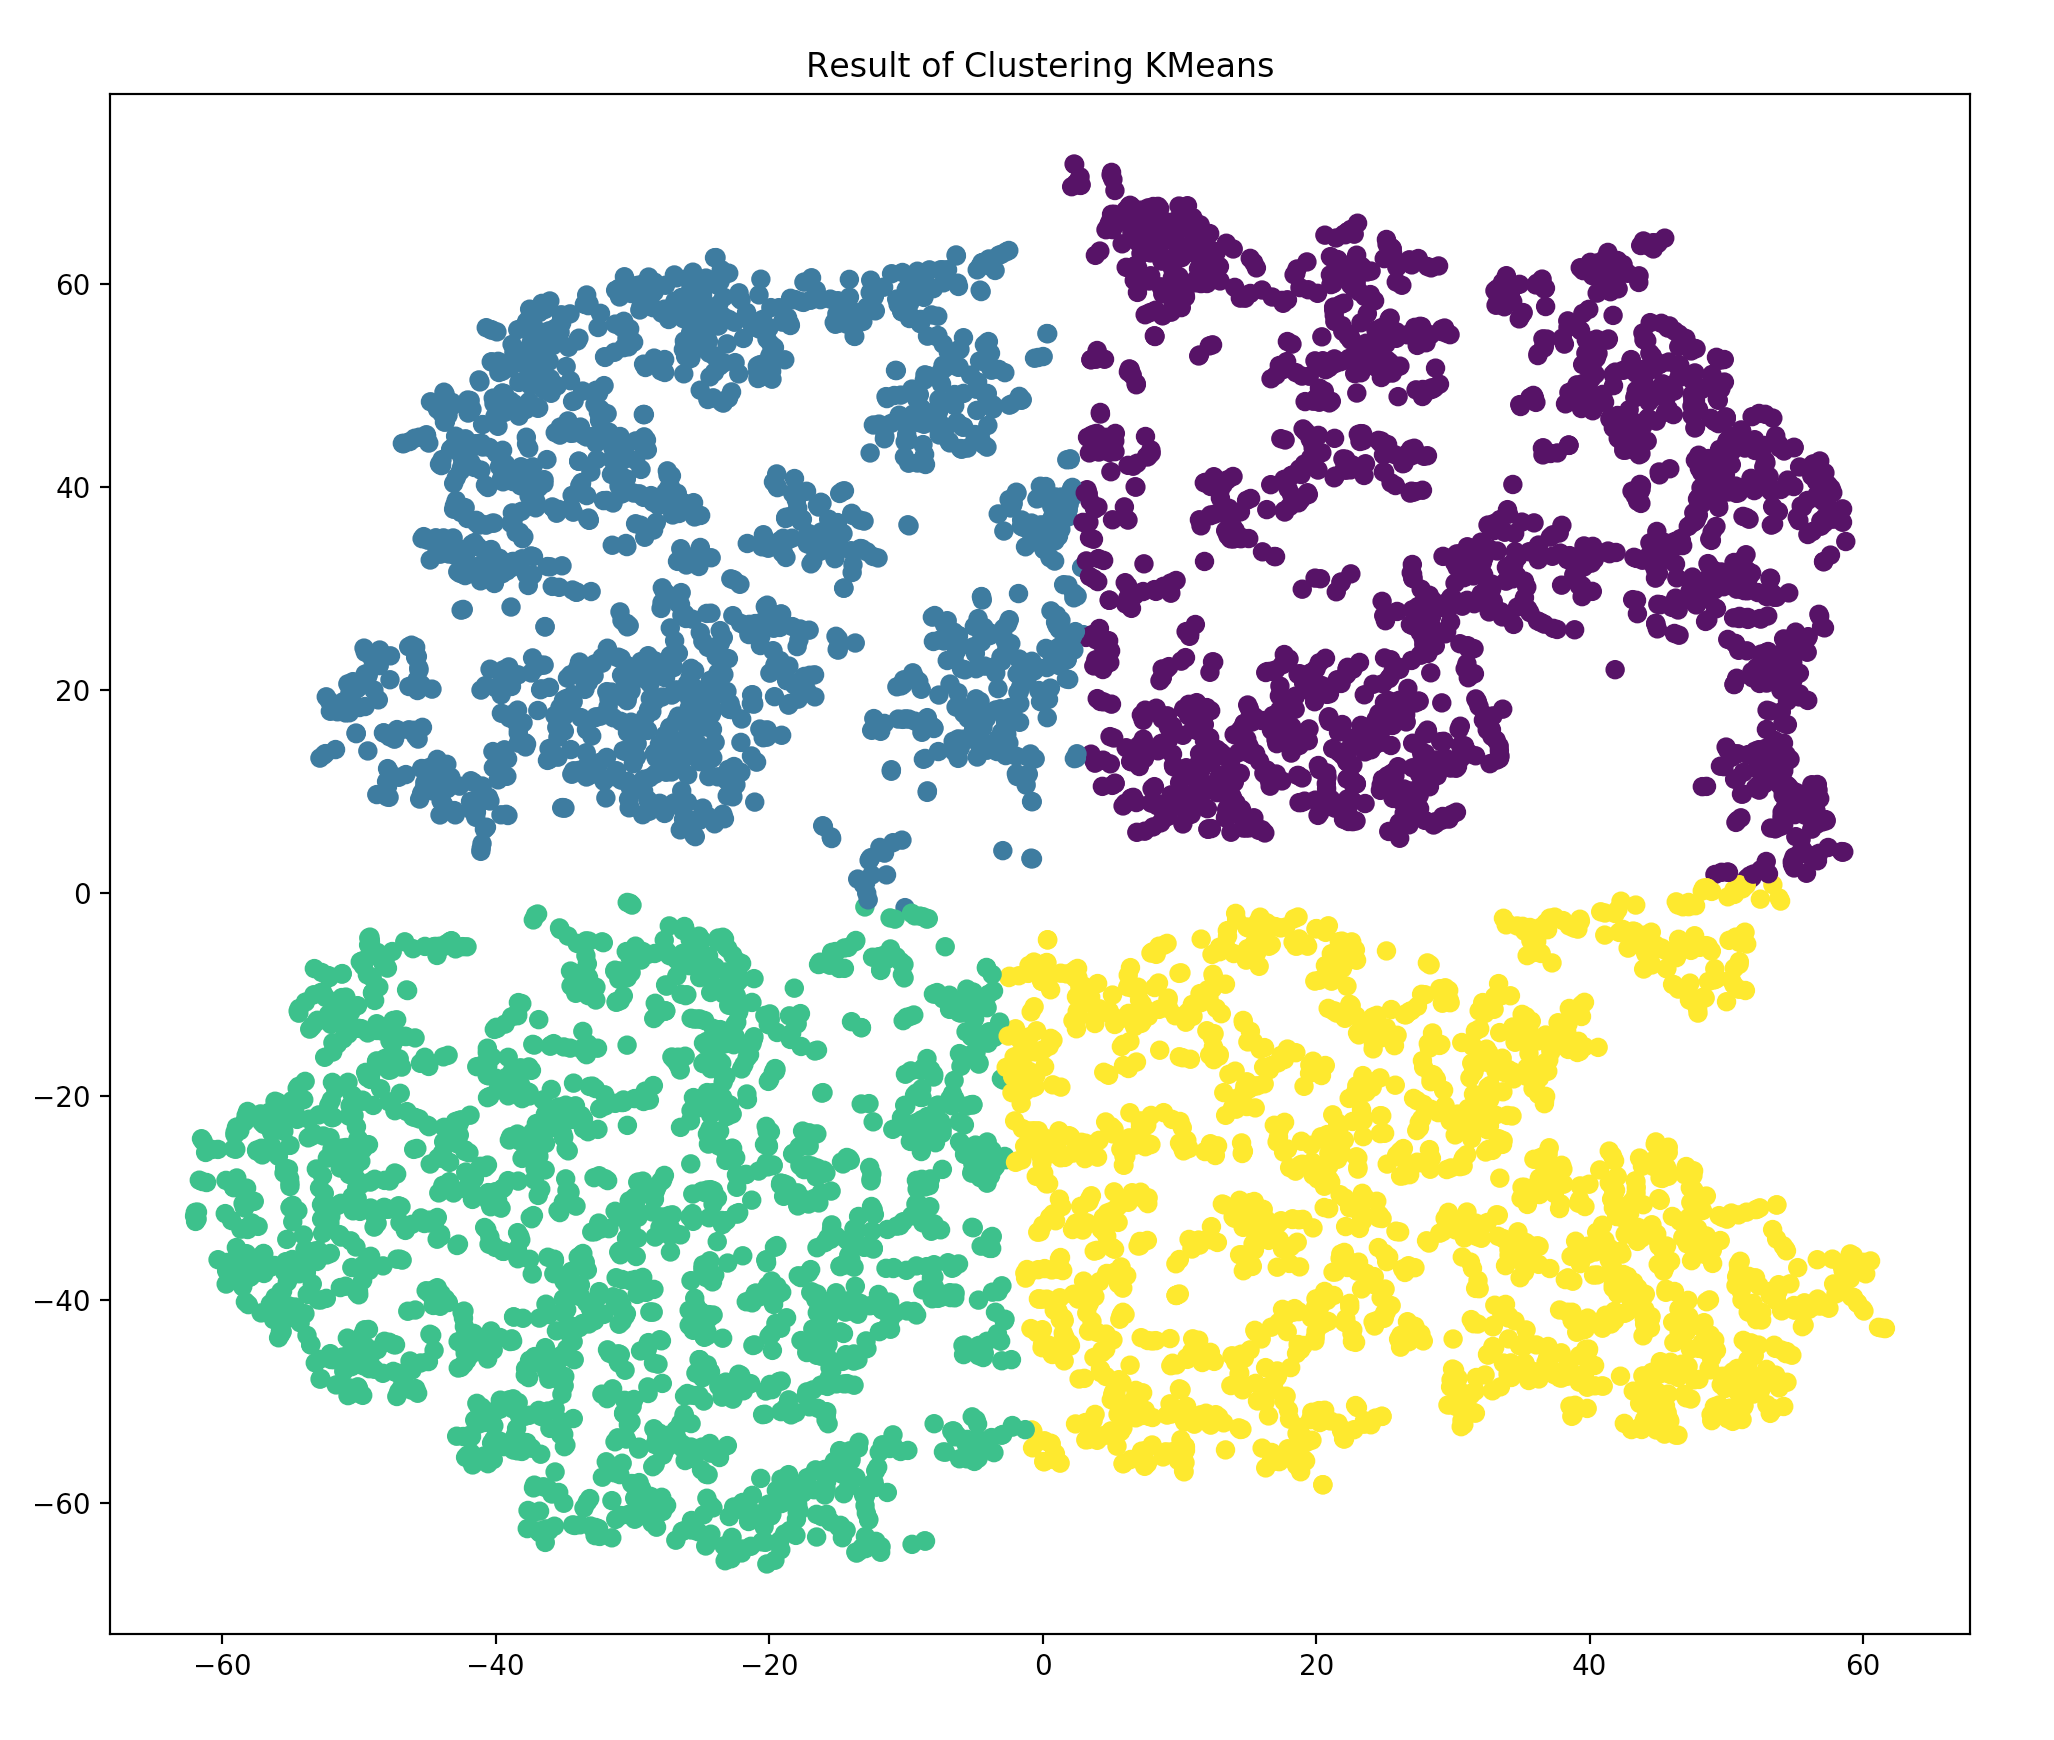
\includegraphics[width=0.4\textwidth]{2-2.png}
    \end{figure}
\end{itemize}

原因分析:

使用特征组合2时聚类效果有一定提升,这是由于特征组合2是由PCA进行降维之后再去训练模型,提升了训练集的可靠性。

此外KMeans的聚类效果优于Birch,这是由于Birch更适用于k值较大,即簇类较多的情况,此处使用的$k=4$,故聚类效果较差。

% That's all folks!
\end{document}
